\section{Fourier series}

\subsection{Continuous Fourier series}
The set set of functions for $k \in \mathbb Z$
\begin{equation*}
    \phi_k(x) = e^{ikx}
\end{equation*}
is an orthogonal system over the interval $(0,2\pi)$ since
\begin{equation*}
    \int_0^{2\pi} \phi_k \overline \phi_l = 2\pi \delta_{kl}.
\end{equation*}
For $u : (0,2\pi) \to \mathbb C$ we introduce the Fourier coefficients
\begin{equation*}
    \hat u_k = \frac 1 {2\pi} \int_0^{2\pi} u(x) \overline \phi_k(x) dx.
\end{equation*}
The Fourier series is defined as
\begin{equation*}
    Su = \sum_{k=-\infty}^\infty \hat u_k \phi_k.
\end{equation*}
As an approximation we use the trigonometric polynomials
\begin{equation*}
    P_N u = \sum_{k=-N/2}^{N/2-1} \hat u_k \phi_k.
\end{equation*}
Recall that if $u$ is periodic and continuous, then $P_N u \to u$ uniformly in $(0,2\pi)$.
We also define the space
\begin{equation*}
    S_N = \spannedby \{ \phi_k : -N/2 \le k \le N/2 - 1\}.
\end{equation*}
We recall Parseval's identity
\begin{equation*}
    \| u \|_{L^2(0,2\pi)}^2 = 2 \pi \sum_{k=-\infty}^\infty |\hat u_k|^2.
\end{equation*}
Thus
\begin{equation*}
    u = \sum_{k=-\infty}^\infty \hat u_k \phi_k \qquad \forall u \in L^2(0,2\pi).
\end{equation*}

\begin{example}
    Let
    \begin{equation*}
        u(x) = \begin{dcases}
            1 & \text{if } \frac \pi 2 < x \le \frac {3\pi}{2} \\
            0 & \text{otherwise}.
        \end{dcases}
    \end{equation*}
    Then
    \begin{equation*}
        \hat u_k = \begin{dcases}
            \pi                      & \text{if } k = 0                \\
            0                        & \text{if } k \ne 0 \text{ even} \\
            \frac{(-1)^{(k-1)/2}}{k} & \text{if } k \ne 0 \text{ odd.}
        \end{dcases}
    \end{equation*}
\end{example}
We can expand the complex exponential as trigonometric functions
\begin{equation*}
    u(x) = \sum_{k=-\infty}^{\infty} a_k \cos k x + \sum_{k=-\infty}^\infty b_k \sin k x
\end{equation*}
where $\hat u_k = a_k - i b_k$. If $u: (0,2\pi)\to \mathbb R$ then $a_k, b_k \in \mathbb R$. In particular, we observe that $P_N u : (0,2\pi) \to \mathbb R$.

\subsection{Periodic functions}

The Fourier series are specially useful for the periodic setting. Let us define
\begin{equation*}
    C^m_p([a,b]) = \left\{ u\in C^m ([a,b]) : \frac{d^k u}{dx^k}(a) = \frac{d^k u}{dx^k}(b) \text{ for } 0 \le k \le m \right\}.
\end{equation*}
We define
\begin{equation*}
    H^m_p(a,b) = \overline{C^m_p([a,b])}^{H^m(a,b)}.
\end{equation*}
We introduce
\begin{equation*}
    \newnorm{u}_{H_p^m(0,2\pi)} = \left(\sum_{k=-\infty}^{\infty} (1 + |k|^{2m}) |\hat u_k|^2 \right)^{\frac 1 2}.
\end{equation*}
This is an equivalent norm of $H_p^m(0,2\pi)$.
\begin{remark}
    Notice that $L^2_p = L^2$, and hence we do not need to assume that $u$ is periodic for $P_N u$ to converge in $L^2(0,2\pi)$.
\end{remark}


\subsection{Discrete Fourier series}
Let us take
\begin{equation*}
    x_j = \frac{2\pi j}{N} \qquad j \in \{0,\cdots, N-1\}.
\end{equation*}
We define
\begin{equation*}
    \tilde u_k = \frac 1 N \sum_{j=0}^{N-1} u(x_j) \overline \phi_k(x_j), \qquad k \in \{-N/2, \cdots, N/2-1\}.
\end{equation*}
We have the ortoganility relation
\begin{equation*}
    \frac 1 N \sum_{j=0}^{N-1}  \phi_l(x_j) \overline \phi_k(x_j) = \frac 1 N \sum_{j=0}^{N-1} e^{i(l - m)x_j} = \begin{dcases}
        1 & l - m \in N \mathbb Z , \\
        0 & \text{otherwise}
    \end{dcases},
\end{equation*}
Thus, we have that
\begin{equation*}
    u(x_j) = \sum_{k=-N/2}^{N/2-1} \tilde u_k \phi_k(x_j), \qquad j \in \{0, \cdots, N-1\}.
\end{equation*}
We set
\begin{equation*}
    I_N u (x) = \sum_{j=0}^{N-1} u(x_j) \psi_j (x), \qquad \text{where } \psi_j (x) = \frac 1 N \sum_{k=-N/2}^{N/2 - 1} \phi_k(x-x_j).
\end{equation*}
We point out that $\psi_j (x_l) = \delta_{lj}$.

\bigskip

Lastly we define the error
\begin{equation*}
    R_N u = \sum_{k=-N/2}^{N/2-1} \phi_k \sum_{\substack{m =-\infty \\ m \ne 0}}^{\infty} \hat u_{k + Nm}
\end{equation*}
We have that $I_N u = P_N u + R_N u$ and
\begin{equation}
    \|u - I_N u\|^2_{L^2(0,2\pi)} = \|u - P_N u\|^2_{L^2(0,2\pi)} + \|R_N u\|^2_{L^2(0,2\pi)}.
\end{equation}

\subsection{Differentiation}
We define the Fourier interpolation derivative of $u$
\begin{equation*}
    \mathcal D_N u \defeq \frac{d}{dx} (I_N u).
\end{equation*}
It does not coincide, in general, with $P_N \frac{du}{dx}$ or $I_N \frac{du}{dx}$.

\subsection{Gibbs' phenomenon}

The Fourier series of a discontinuous function can have oscillations near the discontinuity, see \Cref{fig:Gibbs}
\begin{figure}[H]
    \centering
    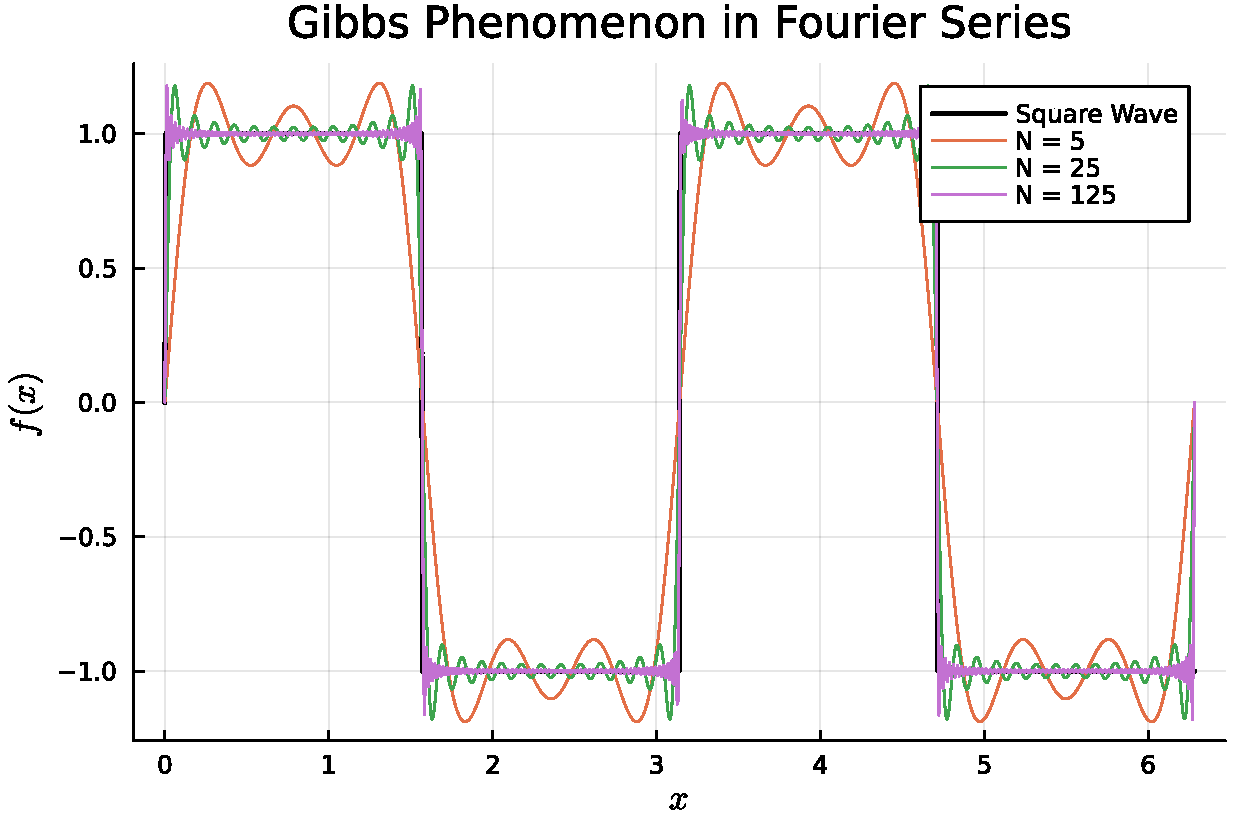
\includegraphics[width=0.5\textwidth]{Gibbs}
    \caption{Gibb's phenomenon}
    \label{fig:Gibbs}
\end{figure}

\subsection{Truncation errors}

\begin{theorem}[Truncation of the Fourier series for a periodic function]
    \label{thm:Fourier truncation of periodic function}
    We have that for $u \in H_p^m (0,2\pi)$ and $k \le m$
    \begin{equation*}
        \|u - P_N u\|_{H^k(0,2\pi)} \le C N^{k-m} \|u^{(m)}\|_{L^2(0,2\pi)}.
    \end{equation*}
\end{theorem}
\begin{proof}
    We prove only the case $k = 0$ for simplicity
    \begin{align*}
        \frac 1 {{2\pi}}  \|u - P_N u\|_{L^2(0,2\pi)}^2
         & =
        \sum_{|k| > N} |\hat{u}_k|^2
        = \sum_{|k| > N} \frac{1}{|k|^{2m}} |k|^{2m} |\hat{u}_k|^2
        \\
         & \leq N^{-2m} \sum_{|k| > N} |k|^{2m} |\hat{u}_k|^2 .\qedhere
    \end{align*}
\end{proof}
As a consequence
\begin{equation*}
    \inf_{\phi \in S_N} \|u - \phi\|_{H^k(0,2\pi)} \le C N^{k-m} \|u^{(m)}\|_{H^m(0,2\pi)}, \qquad \forall u \in H^{m}_p(0,2\pi).
\end{equation*}
We can also prove that
\begin{equation*}
    \|R_N u\|_{L^2} \le C N^{-m} \|u^{(m)} \|_{L^2(0,2\pi)}, \qquad u \in H^{m}_p(0,2\pi).
\end{equation*}

Now is a good time to
\begin{example}[Laplace equation with periodic conditions via Fourier-Galerkin]
    \label{eq:Laplace equation by Fourier-Galerkin}
    Let us assume we are trying to solve
    \begin{equation*}
        \begin{dcases}
            -\Delta u = f & \text{in } (0,2\pi) \\
            u(0) = u(2\pi).
        \end{dcases}
    \end{equation*}
    We need to assume the compatibility condition $\int_0^{2\pi} f = 0$. Notice that this is exactly $\hat f_0 = 0$.
    This problem in under-determined since for any solution $u$, for any constant $c \in \mathbb R$ we have that $u + c$ is also a solution.
    So we look for the solution with $\int_0^{2\pi} u = 0$.
    We extend $u, f: (0,2\pi) \to \mathbb C$ by their Fourier series.
    Thus, we consider
    \begin{equation*}
        V = \left\{ u \in H^1_p(0,2\pi) : \int_0^{2\pi} u = 0 \right\}.
    \end{equation*}
    The problem can be written equivalently as finding $u \in V$ such that
    \begin{equation*}
        (-\Delta u, \phi)_{L^2(0,2\pi)} = (f, \phi)_{L^2(0,2\pi)} , \qquad \forall \phi \in V.
    \end{equation*}
    We point out that $-\Delta \phi_k = k^2 \phi_k$. Using $\phi = \phi_k$ we recover
    \begin{equation*}
        k^2 \widehat u_k = \widehat f_k.
    \end{equation*}
    This is precisely why we need $\widehat f_0 = 0$.
    We can see that the exact solution is
    \begin{equation*}
        u = \sum_{\substack{k=-\infty \\ k \ne 0}}^\infty \frac{\hat f_k}{k^2} \phi_k.
    \end{equation*}
    The corresponding Galerkin problem consists of finding a solution $u_N \in S_N \cap V$ in the sense that
    \begin{equation*}
        (-\Delta u_N, \phi)_{L^2(0,2\pi)} = (f, \phi)_{L^2(0,2\pi)} , \qquad \forall \phi \in S_N \cap V.
    \end{equation*}
    Similarly to before, we observe that
    \begin{equation*}
        u_N = \sum_{\substack{k=-N/2 \\ k \ne 0}}^{N/2-1}\frac{\hat f_k}{k^2} \phi_k = P_N u.
    \end{equation*}
    We can therefore directly estimate the error using \Cref{thm:Fourier truncation of periodic function}.
    Higher orders of convergence require $f \in H^m_p(0,2\pi)$.
\end{example}

\begin{remark}[\Cref{eq:Laplace equation by Fourier-Galerkin} in terms of Céa's lemma]
    Let us define for $u,v$ periodic
    \begin{equation*}
        a(u,v) = (-\Delta u, v)_{L^2(0,2\pi)} = \int_0^{2\pi} \frac{du}{dx} \frac{dv}{dx}
    \end{equation*}
    Due to the Poincaré-Wirtinger inequality this is a coercive bilinear form of $V = H^1_p (0,2\pi; \mathbb R)$. The weak formulation is given by \eqref{eq:Galerkin elliptic variational}
    Let us define $h = N^{-1}$, we can set $V_h = V \cap S_N$.
    Let $u_h \in V_h$ solve \eqref{eq:Galerkin elliptic variational discrete}.
    Again notice that, since this is a very simple example, $u_h = u_N$.
    Then, due to \namedCref{lem:cea} we have that
    \begin{align*}
        \|u - u_h\|_{H^1(0,2\pi)} & \le \|u - P_Nu\|_{H^1(0,2\pi)} \le C h^{(m+2)-1} \|\tfrac{d^{m+2} u}{dx^{m+2}}\|_{L^2(0,2\pi)} \\
                                  & = C h^{m+1} \| \tfrac{d^m f}{dx^m} \|_{L^2(0,2\pi)}.
    \end{align*}
    And by \Cref{lem:Aubin-Nietsche} we have also that
    \begin{align*}
        \|u - u_h\|_{L^2(0,2\pi)} & \le C h^{2} \| f \|_{L^2(0,2\pi)}.
    \end{align*}
\end{remark}

\subsection*{Exercises}

\begin{exercises}
\ex[]
Code the Fourier-Galerkin method in \Cref{eq:Laplace equation by Fourier-Galerkin}. You will need to numerically approximate $\widehat f_k$.
We will discuss numerical integration in the next class.
You avoid this difficulty by using library for numerical integration. In \texttt{julia} you can use \texttt{Integrals.jl}.

Code the corresponding Fourier-colocation method using the points $x_j = 2\pi j / N$ for $j = 0, \cdots, N-1$.

Compare the numerical errors as a function of $N$.
\end{exercises}